\chapter{Development}
\paragraph{Stage 1 - project start}   
\addtocounter{section}{1}
\addcontentsline{toc}{section}{
    \protect\numberline{\thesection} Stage 1 - project start}
\mbox{}\\
The first phase development process was greatly filled up with waiting. I joined the project in February when the project was still only on paper, teams were formed to perform certain tasks and we began ordering of necessary parts.

Having experience with similar systems I instantly realised that a National Instruments' controller we had in-house would be a good choice for the main control unit. CompactRIO - the family name of the controller, consist a variety of devices within fast and reliable real-time processor thigh up within FPGA (Field-Programmable Gate Array) all packaged intro rugged industrial form\footnote{One of the packaging options}.

From the variety of options, I have chosen model cRIO9033 which has a great proportion between the performance and size. It comes with the following relevant parameters:
\begin{table}[H]
    \centering
    \begin{tabular}{r|c}
        Processor & Dual Core Intel Atom E3825 (1.33 GHz) \\
        RAM & 2GB (DDR3L) \\
        FPGA & Xilinx Kintex-7 7K160T \\
        Extension slots & 4
    \end{tabular}
    \caption*{}
    \label{tab:cRIO_param}
    \vspace{-20pt}
\end{table}

As a consequence, the software needed to be written in LabVIEW (G - language). LabVIEW has a strong position in the industry being used some great project like Space X or CERN, moreover, it has been widely adopted also in the automotive industry by companies as:
\begin{table}[H]
    \centering
    \begin{tabular}{c|c|c|c|c}
        Audi & Toyota & Nissan & Honda & Bosh \\ 
        Continental & Delphi & Visteon & DaimlerChrysler & Autoliv \\
        Land Rover & Jaguar & BMW & Volkswagen & TRW \\
        General Motors & Eaton Corp & Lear Corp & Saab & Ford \\
        Siemens VDO & Breed Technologies & Fiat & Magneti Marelli & Ferrari \\
        Skoda & Suzuki & Valeo & Volvo & ...
    \end{tabular}
    \caption*{\cite{LabVIEW_adoption}}
    \label{tab:LabVIEW_adoption}
\end{table}
With this in mind, although, being unfamiliar with its graphical programming interface at first, I was glad to have opportunity to study it in depth.

For the first two months I have been studying the topic, learning the LabVIEW usage and preparing conceptual software implementation, yet not having any device it could communicate with.

\paragraph{Stage 2 - arrival of key components}   
\addtocounter{section}{1}
\addcontentsline{toc}{section}{
    \protect\numberline{\thesection} Stage 2 - arrival of key components}
\mbox{}\\
In the second week of April, I have been given an early prototype of CAN peripheral device which simply been sending a repetitive message containing a value of running counter. As a basic test prototype has been proved to successfully transmit CAN message in between two Arduinos (development boards used as CAN peripherals). Therefore I assumed it works correctly, however, I was not capable to read the message by cRIO. After a few weeks of debugging, I discovered that peripheral transmission speed was off from desired and send it for revision.

Meanwhile, in the third week of April, the motor controllers arrived. So as soon as it happened I have made myself connection to interface with them. Although, available non of libraries was providing full functionality for CANOpen implementation based on used NI9853 CAN module. As implementing this solution from the ground up would be far out of scope for this thesis, the decision was made on acquiring additional module designed implicitly for CANOpen communication (NI9881).

Concurrently, also the BMS arrived so I have made a physical connection and powered it up, however, the bus voltage was floating showing only electromagnetic noise, therefore, I decided to wait until responsible team would be able to setup initial configuration of this device.

\paragraph{Stage 3 - Implementation}   
\addtocounter{section}{1}
\addcontentsline{toc}{section}{
    \protect\numberline{\thesection} Stage 3 - Implementation}
\mbox{}\\
In the mid-May just a week after the arrival of the NI9881 module and receiving a working peripheral prototype, I had both protocols running. I started by implementing a basic logging feature and tried to control the state of the motor controller. 

Although basic communication was set there was still a lot of work to be done, I dedicated my time to setup configuration of motor controller and write the library(\ref{SDO_wrappers}) to be able to control it in convenient, declarative way.
It was a great challenge as controller documentation was incomplete and momentary misleading. First of all, I found the way to set up the parameters, however from there to spin up the motors the path was not so straightforward. 
The motor controller uses two parallel state machines, one which is based on CANOpen standard and second which has been implemented by the manufacturer (\ref{fig:em500_states}). 
\begin{figure}[H]
    \centering
    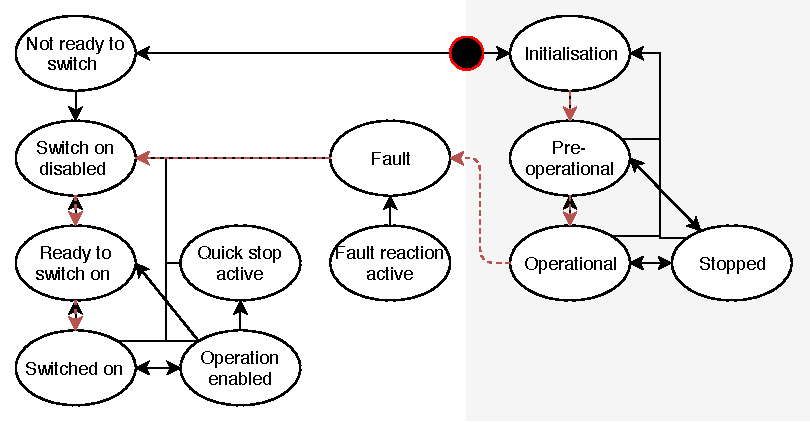
\includegraphics[width=0.8\textwidth]{figures/em500_state}
    \caption{emDrive500 states machines correlation}
    \label{fig:em500_states}
\end{figure}\todo{correct arrow colour to op en}
Although, it is not described in the manual these two state machines are correlated. After many, many tries I decided to closely follow the steps I found in an unofficial manual. It turned out to be a successful approach. 

In figure \ref{fig:em500_states} I have marked by red arrows the only way to boot device into the operational state. Moreover, what could not be shown in the figure in CANOpen's pre-operational state not officially documented parameter\footnote{Currently available manual does not provide description for objects with addresses starting with 0x3000} needed to be set to choose control mode (torque/speed). This founding allowed me to make a step forward, by being able to spin the motor.
Advancing the testing program lead me to the point where to reduce protocol overhead I implemented control based on default PDO messages. It has been able to read motor controller status within an interval of one millisecond, simultaneously controlling the target speed.

Counting it as success I moved my focus towards communication with other peripherals. I got delivered a very first version of the pedal position smart sensor but it has not been at the time working properly.
\begin{itemize}
    \item In case of errors random position values were send
    \item There was no documentation about how errors are encoded (little/big-endian, byte order)
    \item The calibration process was way over-complicated (press calibration button for each limit of control)
    \item Readings were useless, whenever the motors were on due to high electromagnetic noise
\end{itemize} 
I took my time and tried to debug/improve it with a responsible team. After many iterations, we finally came up with a solution which did not have any of the above-mentioned problems.

Willing to integrate all implementations so far and start working on an electrical differential setup I have tried to control two motors simultaneously. This seemingly small step turned out to be a problematic in implementation.
As the control of motors has been based on PDO protocol to be capable to control two motors independently on the same bus the message IDs of at least one motor controller needed to be changed. I have written the code to do so, however it did not work as desired. Being completely confused I spend few days debugging the issue. 
It turned out, although, proper commands have been issued the controller would just accept them without changing anything. I had a hard time to believe that the device might malfunction this way yet there was no other explanation. Therefore, I contacted the manufacturer which right away admit that he is aware of this software bug and provided instruction and new software version to solve the issue. However that was not the end of the problems.
After the software was uploaded the device stopped booting so just two and half weeks before competition it needed to be sent for repair. It has been done within about the week, however, POD protocol remain unusable.
To overcome this problem in place of PDO commands the slower SDO protocol has been used. Although message frequency needed to be limited, this solution proved to provide just sufficient performance.

About the time also I have been helping with pump controlling module and worked on gathering everything into the consistent system which has been comprehensively described in the next chapter.